\documentclass[12pt,oneside]{book} % for one-sided printing

\usepackage{blindtext}% Just used so we can generate some example text
\usepackage{amsmath}
\usepackage{algorithm}
\usepackage{algpseudocode}
\usepackage{amssymb}
\usepackage{mathtools}
\usepackage[export]{adjustbox}
\usepackage{lipsum}
\usepackage{booktabs}  % For better quality tables
\usepackage{longtable} % Pour les tableaux sur plusieurs pages
\usepackage{tabularx}  % for the X column type
\usepackage{listings}
\usepackage{xcolor}
\usepackage{caption}
\usepackage{xfrac}
\usepackage{indentfirst}
\usepackage{subcaption}
\usepackage{graphicx}
\usepackage{geometry}
\geometry{a4paper, margin=1in}

% Place style file after other packages.
\usepackage{cranfieldthesis}
\usepackage{lscape} % for landscape pages
\usepackage{float}
\usepackage[toc,title,page]{appendix}

% Couleurs personnalisées
\definecolor{backcolour}{rgb}{0.96, 0.96, 0.96} % Fond très clair
\definecolor{codegray}{rgb}{0.47, 0.47, 0.47}   % Commentaires et numéros de ligne
\definecolor{codegreen}{rgb}{0.25, 0.50, 0.35}  % Commentaires
\definecolor{codeblue}{rgb}{0.26, 0.44, 0.58}   % Mots-clés
\definecolor{codepurple}{rgb}{0.50, 0, 0.50}    % Identificateurs
\definecolor{codeteal}{rgb}{0, 0.5, 0.5}        % Chaînes de caractères
\definecolor{terminalback}{rgb}{0.05, 0.05, 0.05} % Fond très sombre pour le terminal
\definecolor{terminaltext}{rgb}{0.7, 0.7, 0.7}    % Texte clair pour le terminal
\definecolor{mygreen}{rgb}{0,0.6,0}
\definecolor{mygray}{rgb}{0.5,0.5,0.5}
\definecolor{mymauve}{rgb}{0.58,0,0.82}
\definecolor{terminalbgcolor}{HTML}{330033}
\definecolor{terminalrulecolor}{HTML}{000099}

\lstdefinestyle{bashstyle}{
    language=bash,
    backgroundcolor=\color{backcolour},
    basicstyle=\ttfamily\scriptsize,
    keywordstyle=\color{blue},
    stringstyle=\color{red},
    identifierstyle=\color{codepurple},
    commentstyle=\color{codegreen},
    morecomment=[l]{\#},   % Define comment style
    frame=single,          % adds a frame around the code
    rulecolor=\color{gray},% if not set, the frame-color may be changed on line-breaks
    breakatwhitespace=false,
    breaklines=true,       % sets automatic line breaking
    captionpos=b,          % sets the caption-position to bottom
    keepspaces=true,       % keeps spaces in text
    showspaces=false,      % show spaces everywhere adding particular underscores
    showstringspaces=false % underline spaces within strings only
}

\lstdefinestyle{cstyle}{
    language=C++,
    basicstyle=\ttfamily\scriptsize,
    keywordstyle=\color{blue},
    backgroundcolor=\color{backcolour},
    stringstyle=\color{red},
    commentstyle=\color{codegreen},
    morecomment=[l][\color{magenta}]{\#},
    breaklines=true,
    numbers=left,
    numberstyle=\tiny\color{gray},
    showstringspaces=false,
    tabsize=2,
    frame=single
}

% Title Page Set Up
\title{Artificial Intelligence Assignment}
\author{Alexis Balayre}
\date{18\textsuperscript{th} March 2024}
\school{\SATM}
\degree{MSc}
\course{Computational Software of Techniques Engineering}
\academicyear{2023 - 2024}

% Supervisors
\supervisor{Dr Jun Li}

% Copyright
\copyrightyear{2024}

% References
\usepackage[numbers]{natbib} % for nice referencing
\makeatletter % Reference list option change to number and period
\renewcommand\@biblabel[1]{#1.} % from [1] to 1
\makeatother %
\setcitestyle{round} % use round citations

\begin{document}

\frontmatter

% Form Title Pages
\maketitle

% Abstract and Keywords
\begin{abstract}

    High-Performance Computing (HPC) systems are pivotal in solving complex
    computational problems. Leveraging such systems, this report investigates the
    optimization of sparse matrix-vector multiplication (SpMV) - a crucial
    operation in scientific computations. Two prevalent storage formats, Compressed
    Sparse Row (CSR) and ELLPACK, are parallelized using OpenMP and CUDA to enhance
    SpMV's efficiency on the CRESCENT2 HPC cluster at Cranfield University.

    The study reveals that CSR format, when parallelized with OpenMP, achieves
    superior performance across a majority of matrices due to efficient memory
    management and task distribution. CUDA parallelization exhibits significant
    speed-ups, especially for matrices with regular structures, indicating an
    intricate relationship between matrix properties and the efficiency of CSR and
    ELLPACK formats.

    Experimental results suggest that the parallelization strategy should be
    selected based on matrix characteristics. For matrices with high density or
    regularity, CUDA outperforms OpenMP, whereas for less regular matrices, OpenMP
    provides sufficient speed-up. Sequential execution remains competitive for
    small matrices or those with unfavourable characteristics for parallelization.

    This report underscores the necessity of aligning parallel programming
    strategies with matrix properties to fully exploit HPC capabilities, providing
    a foundation for future research towards more nuanced and effective
    computational techniques in scientific computing.

\end{abstract}

% Use single spacing for Table of Contents, List of Figures, etc
{
\clearpage
\singlespacing
% Table of Contents
{
    \tableofcontents
}
\clearpage

% List of Figures
\listoffigures

% List of Tables
\listoftables
}

%% Main Matter
\mainmatter
\pagestyle{fancy}
\fancyhead[L]{\nouppercase{\leftmark}}
\fancyhead[R]{\nouppercase{\rightmark}}

\chapter{Introduction}

Accurately diagnosing thoracic abnormalities from radiographs (X-rays)
represents a considerable challenge, even for experienced radiologists. The
complexity and critical nature of diagnosing these anomalies requires
increasingly sophisticated decision support tools. In this context, the
competition organised by Vingroup's Big Data Institute, supported by Vingroup
JSC and launched in August 2018, aims to promote fundamental research in data
science and artificial intelligence, with a particular focus on medical image
processing.

The main objective of the competition is to develop automated systems capable
of locating and classifying 14 types of thoracic anomalies from chest X-ray
images.This initiative underlines the need for greater precision in medical
diagnosis, where current methods struggle in particular to specify the location
of findings on X-ray images, potentially leading to incorrect diagnoses.

\section{Problem Statement}

\section{Dataset}

The dataset provided to participants includes 18,000 annotated chest scans, of
which 15,000 images are for training and 3,000 for evaluation. These
annotations were carefully collected via VinBigData's VinLab platform from
de-identified studies provided by two Vietnamese hospitals.

\section{Significance of the Competition}

This competition promises significant advances in medical diagnosis by
potentially providing radiologists with a reliable secondary opinion. By
automating the detection and location of chest X-ray findings, the solution
aims to lighten the workload of healthcare professionals and improve diagnostic
accuracy for patients, particularly benefiting those in resource-limited
settings.

\section{Evaluation Metric}

The competition uses the PASCAL VOC 2010 Mean Average Precision (mAP) metric
with an Intersection on Union (IoU) threshold of >0.4 to evaluate submissions.
This metric highlights the importance of accuracy in the detection and
classification process.

\chapter{literature Review}

Object detection is a fundamental task in computer vision that involves
identifying and locating objects of different categories in an image or video.
Unlike image classification, which assigns a label to the entire image, object
detection aims to provide a label and bounding box for each object of interest
in the image.

\section{Basic principles}

Object detection generally involves two main tasks: object classification
(knowing what objects are) and object localisation (knowing where objects are).
To be successful, an object detection system must be able to recognise objects
under a variety of conditions, such as different sizes, viewing angles, and
occlusion levels.

\section{Object Detection Technologies}

\subsection{Convolutional Neural Networks (CNN)}

CNNs are at the heart of many advances in object detection. They are
particularly effective at extracting hierarchical features from images thanks
to their layered structure, which includes convolutional layers, pooling layers
and fully connected layers.

\subsection{Region-based approaches}

\subsubsection{R-CNN}

R-CNN (Regions with CNN features) uses proposed regions to identify potentially
interesting parts of the image, then applies a CNN to each of these proposed
regions to classify the objects.

\subsubsection{Fast R-CNN}

Fast R-CNN improves on R-CNN by using a more efficient architecture that shares
convolution calculations across the entire image, reducing processing time.

\subsubsection{Faster R-CNN}

Faster R-CNN introduces a Region Proposal Network (RPN) that generates region
proposals directly from image features, further improving detection speed and
accuracy.

\subsection{Single Processing Methods}

\subsubsection{YOLO (You Only Look Once)}

YOLO divides the image into a grid and predicts bounding boxes and class
probabilities for each grid cell in a single pass, offering high processing
speed.

\subsubsection{SSD (Single Shot MultiBox Detector)}

SSD combines the advantages of region-based approaches and single-shot methods,
using bounding boxes at different scales and aspect ratios to predict the
presence of objects in the image.

\chapter{Methodology}

\section{Data Exploration}

\begin{figure}[H]
    \centering
    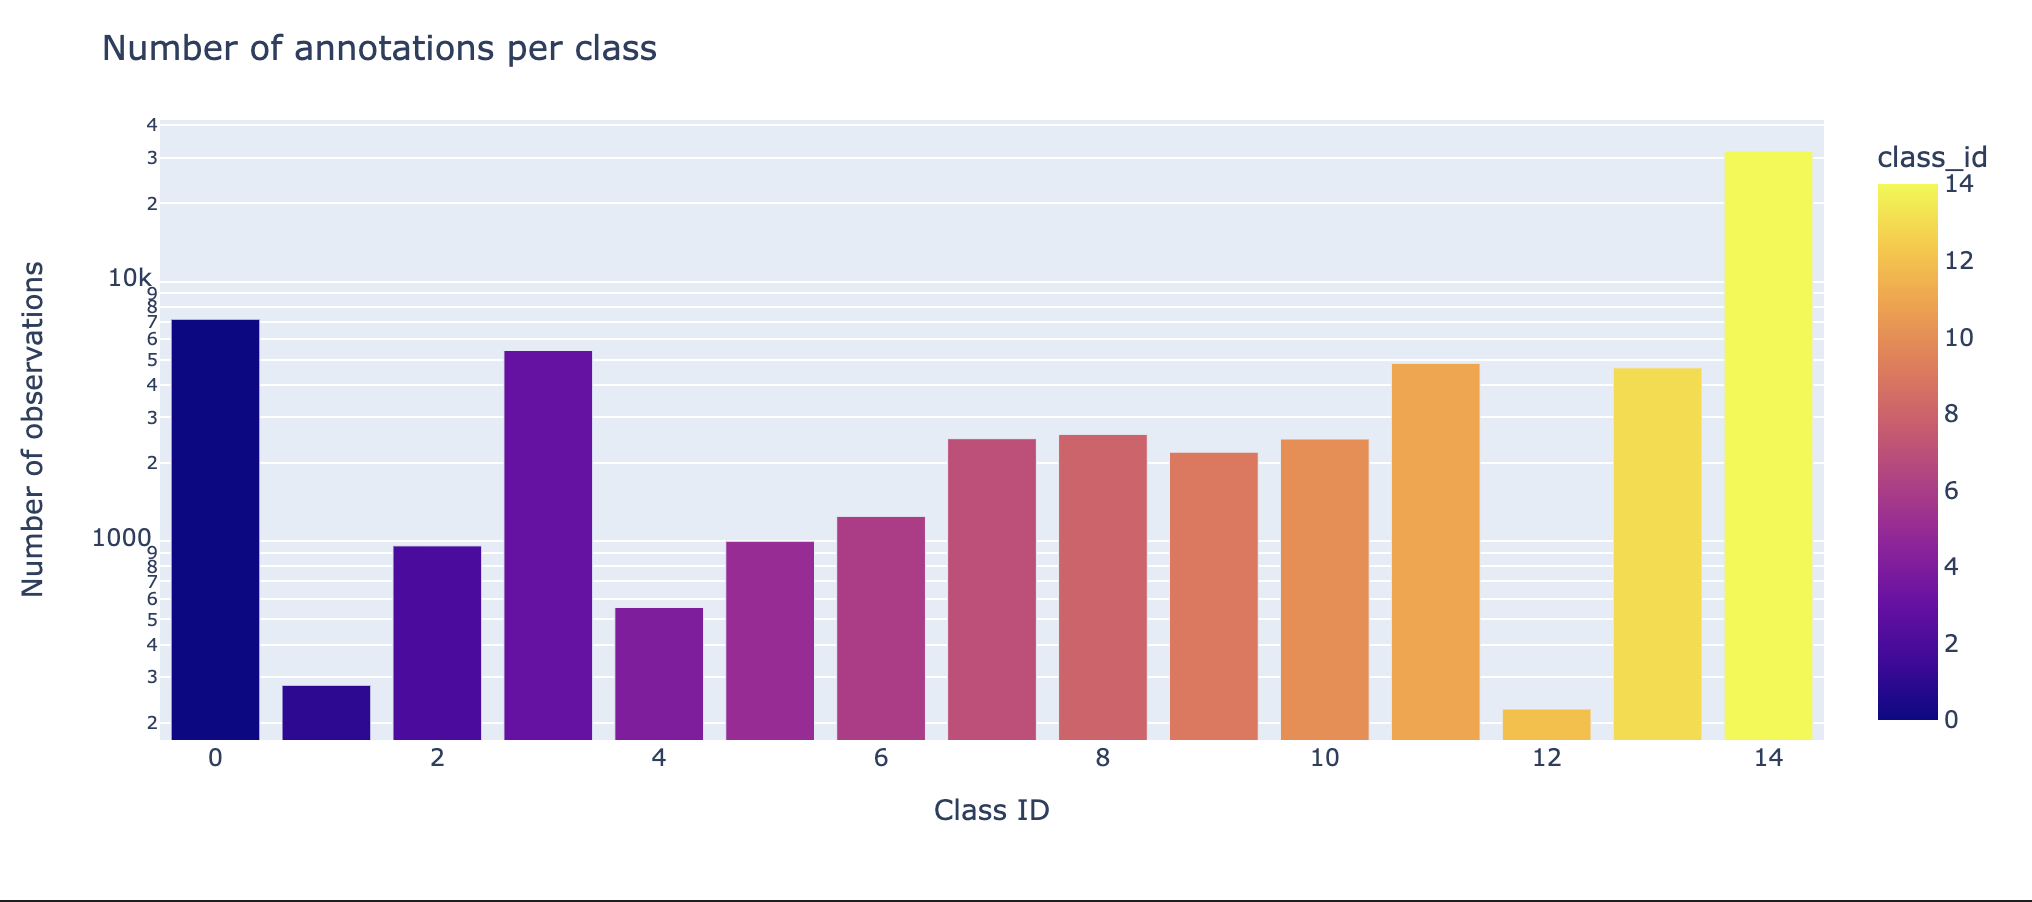
\includegraphics[width=0.8\textwidth]{../results/annotations_per_class.png}
    \caption{Distribution of annotations per class}
    \label{fig:annotations_per_class}
\end{figure}

\begin{figure}[H]
    \centering
    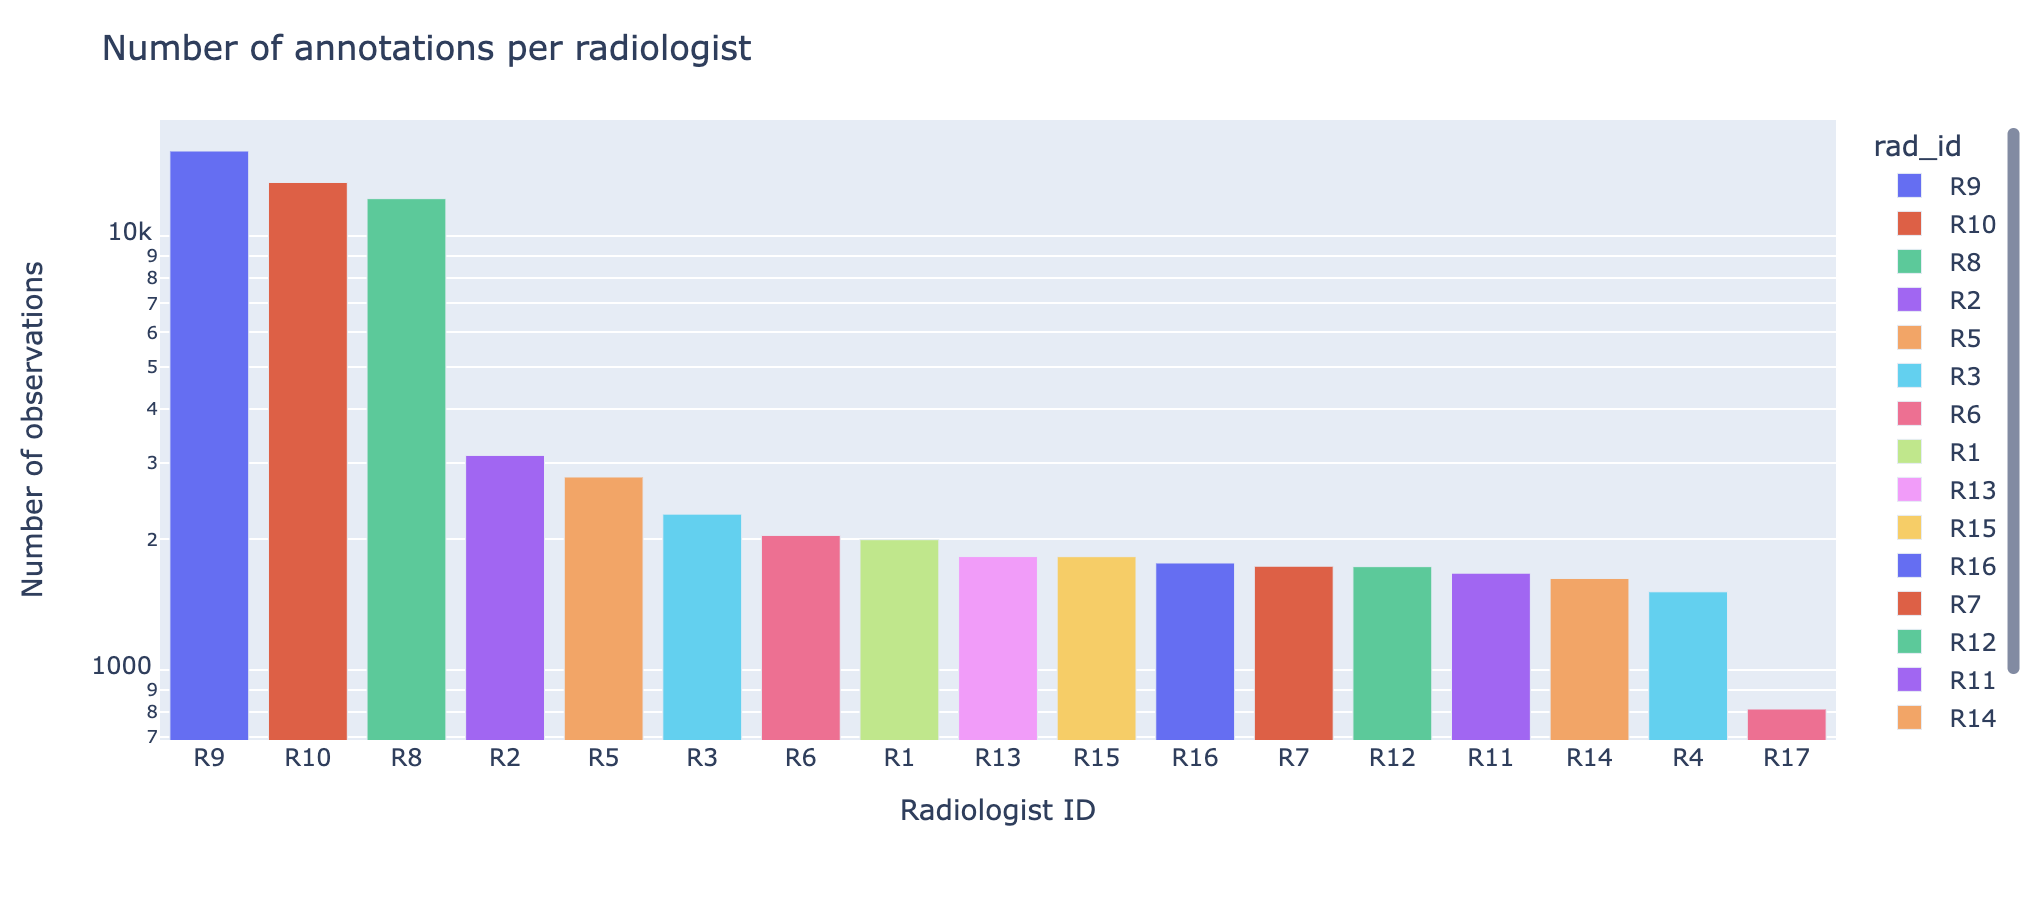
\includegraphics[width=0.8\textwidth]{../results/annotations_per_rad.png}
    \caption{Distribution of annotations per radiologist}
    \label{fig:aannotations_per_rad}
\end{figure}

\begin{figure}[H]
    \centering
    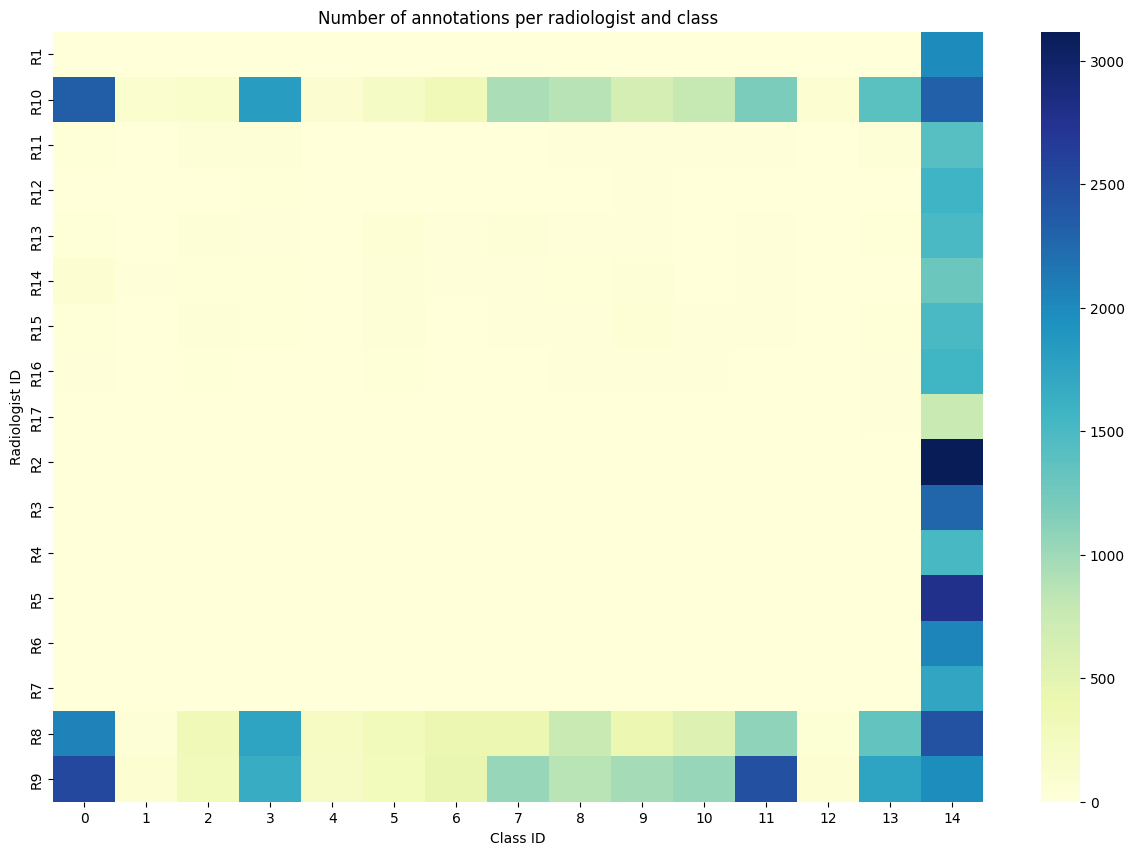
\includegraphics[width=0.8\textwidth]{../results/annotations_per_rad_class.png}
    \caption{Distribution of annotations per image}
    \label{fig:annotations_per_rad_class}
\end{figure}

\section{Data Extraction and Preprocessing}
\subsection{DICOM files Metadata Extraction}

\subsection{DICOM images preprocessing and extraction}

\subsection{DICOM images features extraction}

\section{Evaluation metrics for Faster R-CNN}

To evaluate the performance of the Faster R-CNN model in the object detection
task task, several metrics are used. These metrics provide a quantitative
measure of the model's ability to correctly identify and locate objects in
images.

\subsection{Intersection over Union (IoU)}

Intersection over Union (IoU) is a key metric for assessing the accuracy of of
the bounding boxes predicted by the model. It is defined as the ratio between
the area of the intersection and the area of the union of the predicted and
ground truth:

\begin{equation}
    IoU = \frac{\text{Intersection area}}{\text{Union area}}
\end{equation}

A prediction is considered correct if the IoU with a ground truth box field
exceeds a certain threshold, typically set at 0.5.

\subsection{Precision and Recall}

Precision is the proportion of positive identifications that are correct, while
recall is the proportion of actual ground truths that are truths that are
correctly identified. They are calculated as follows:

\begin{equation}
    \text{Precision} = \frac{TP}{TP + FP}
\end{equation}

\begin{equation}
    \text{Recall} = \frac{TP}{TP + FN}
\end{equation}

where $TP$ represents true positives, $FP$ false positives, and $FN$ false
negatives.

\subsection{Mean Average Precision (mAP)}

The mean Average Precision (mAP) is the average of the APs calculated for each
class of objects over different IoU thresholds. The AP for a class is the area
under the precision-recall curve, and the mAP is an average of these values for
all classes:

\begin{equation}
    mAP = \frac{1}{N} \sum_{i=1}^{N} AP_i
\end{equation}

where $N$ is the number of classes and $AP_i$ is the Average Precision for
class $i$.

These metrics provide a comprehensive assessment of the performance of the
Faster R-CNN model, measuring how accurately the model is able to detect and
locate objects in different images.

\chapter{Results and Discussion}
\section{Results}

\subsection{Sequential Algorithms}

The following table shows the performance comparison of the sequential
algorithms using the CRS and ELLPACK formats.

%TC:ignore
\begin{longtable}{lcccr}
    \label{tab:sequential}                                                        \\
    \caption{Performance Comparison of CRS and ELLPACK Sequential Algorithms}     \\
    \toprule
    \textbf{Matrix}   & \textbf{CRS} & \textbf{ELLPACK} & \textbf{Best Structure} \\
    \midrule
    \endfirsthead
    \toprule
    \textbf{Matrix}   & \textbf{CRS} & \textbf{ELLPACK} & \textbf{Best Structure} \\
    \midrule
    \endhead
    \bottomrule
    \endfoot
    Cube\_Coup\_dt0   & 6.313540     & 2.659870         & CRS                     \\
    FEM\_3D\_thermal1 & 5.939650     & 2.543850         & CRS                     \\
    ML\_Laplace       & 6.629070     & 2.775640         & CRS                     \\
    PR02R             & 6.577900     & 2.755250         & CRS                     \\
    adder\_dcop\_32   & 4.481260     & 2.360730         & CRS                     \\
    af23560           & 5.804440     & 2.509250         & CRS                     \\
    af\_1\_k101       & 6.139610     & 2.608660         & CRS                     \\
    amazon0302        & 2.344020     & 0.968039         & CRS                     \\
    bcsstk17          & 6.256790     & 2.654560         & CRS                     \\
    cage4             & 0.871628     & 0.849791         & CRS                     \\
    cant              & 6.419710     & 2.687030         & CRS                     \\
    cavity10          & 6.032170     & 2.625250         & CRS                     \\
    cop20k\_A         & 4.771770     & 2.155300         & CRS                     \\
    dc1               & 4.686860     & 2.349130         & CRS                     \\
    lung2             & 4.634780     & 2.319800         & CRS                     \\
    mac\_econ\_fwd500 & 3.684580     & 1.851230         & CRS                     \\
    mcfe              & 6.069120     & 2.634280         & CRS                     \\
    mhd4800a          & 5.474340     & 2.549000         & CRS                     \\
    mhda416           & 5.524470     & 2.516310         & CRS                     \\
    nlpkkt80          & 5.932140     & 2.567120         & CRS                     \\
    olafu             & 6.481010     & 2.724440         & CRS                     \\
    olm1000           & 4.775320     & 2.192310         & CRS                     \\
    raefsky2          & 6.556030     & 2.767780         & CRS                     \\
    rdist2            & 5.762990     & 2.465300         & CRS                     \\
    roadNet-PA        & 2.721200     & 1.240050         & CRS                     \\
    thermal1          & 4.599780     & 2.228430         & CRS                     \\
    thermal2          & 3.206760     & 1.437750         & CRS                     \\
    thermomech\_TK    & 3.558870     & 1.592880         & CRS                     \\
    webbase-1M        & 3.750440     & 1.888800         & CRS                     \\
    west2021          & 4.184400     & 2.181630         & CRS                     \\
\end{longtable}
%TC:endignore

A few key observations can be made:
\begin{itemize}
    \item \textbf{CRS Dominance:} For the majority of matrices tested, the CRS format systematically outperforms the ELLPACK format. This is evident for matrices such as Cube\_Coup\_dt0, FEM\_3D\_thermal1, and ML\_Laplace, where CRS not only handles large matrices efficiently but also matrices with high average and maximum numbers of non-zero elements per row.
    \item \textbf{Efficiency in Dense Matrices:} The CRS format appears to be particularly efficient at handling high-density matrices (higher AVG NZR and MAX NZR), which could be attributed to its storage efficiency and the way it streamlines the multiplication process for rows with varying lengths of non-zero elements.
\end{itemize}

\newpage
\subsection{OpenMP}
\subsubsection{Chunk Size Analysis}

As shown in Figures~\ref{fig:openmpchunksizecrs} and
\ref{fig:openmpchunksizellpack}, the performance of the OpenMP parallel
algorithms is influenced by the chunk size. For lower density matrices, the
optimal chunk size is 64 for the CRS format and 32 for the ELLPACK format. For
higher density matrices, the optimal chunk size is 128 or 256 for both formats.

\subsubsection{Thread Count Analysis}

As shown in Figures~\ref{fig:openmpthreadscrs} and
\ref{fig:openmpthreadsellpack}, the performance of the OpenMP parallel
algorithms is influenced by the number of threads. As more threads are used,
the performance improves up to a certain point, after which the performance
starts to stagnate due to the overhead of managing the threads.

\subsubsection{Performance Comparison}

%TC:ignore 
\begin{longtable}{lcccr}
    \caption{CRS vs ELLPACK using OpenMP}                                                            \\
    \label{tab:crsvsellpackopenmp}                                                                   \\
    \toprule
    \textbf{Matrix}   & \textbf{CRS} & \textbf{ELLPACK} & \textbf{Best Structure} & \textbf{Speedup} \\
    \midrule
    \endfirsthead
    \toprule
    \textbf{Matrix}   & \textbf{CRS} & \textbf{ELLPACK} & \textbf{Best Structure} & \textbf{Speedup} \\
    \midrule
    \endhead
    \bottomrule
    \endfoot
    Cube\_Coup\_dt0   & 29.0243      & 27.0415          & CRS                     & 4.597152         \\
    FEM\_3D\_thermal1 & 22.5277      & 19.9711          & CRS                     & 3.792766         \\
    ML\_Laplace       & 33.2766      & 31.9121          & CRS                     & 5.019799         \\
    PR02R             & 32.5086      & 30.2968          & CRS                     & 4.942094         \\
    adder\_dcop\_32   & 5.12204      & 4.83417          & CRS                     & 1.142991         \\
    af23560           & 21.7606      & 18.9078          & CRS                     & 3.748958         \\
    af\_1\_k101       & 26.067       & 23.4946          & CRS                     & 4.245709         \\
    amazon0302        & 7.29883      & 5.23835          & CRS                     & 3.113809         \\
    bcsstk17          & 25.5293      & 23.3597          & CRS                     & 4.080255         \\
    cage4             & 0.385164     & 0.334653         & CRS                     & 0.441890         \\
    cant              & 29.7794      & 27.6956          & CRS                     & 4.638745         \\
    cavity10          & 19.0148      & 16.7258          & CRS                     & 3.152232         \\
    cop20k\_A         & 19.5918      & 17.8729          & CRS                     & 4.105772         \\
    dc1               & 10.4524      & 9.39085          & CRS                     & 2.230150         \\
    lung2             & 8.832        & 6.85328          & CRS                     & 1.905592         \\
    mac\_econ\_fwd500 & 10.5515      & 8.84879          & CRS                     & 2.863691         \\
    mcfe              & 12.6097      & 11.8456          & CRS                     & 2.077682         \\
    mhd4800a          & 18.3501      & 16.1582          & CRS                     & 3.352021         \\
    mhda416           & 7.06099      & 6.80262          & CRS                     & 1.278130         \\
    nlpkkt80          & 24.4853      & 21.694           & CRS                     & 4.127566         \\
    olafu             & 29.966       & 27.9111          & CRS                     & 4.623662         \\
    olm1000           & 2.95895      & 2.1558           & CRS                     & 0.619634         \\
    raefsky2          & 27.8548      & 25.7504          & CRS                     & 4.248730         \\
    rdist2            & 15.5283      & 12.2527          & CRS                     & 2.694487         \\
    roadNet-PA        & 4.63584      & 3.01227          & CRS                     & 1.703601         \\
    thermal1          & 11.7254      & 8.83925          & CRS                     & 2.549122         \\
    thermal2          & 8.84723      & 6.75174          & CRS                     & 2.758931         \\
    thermomech\_TK    & 10.9908      & 8.10205          & CRS                     & 3.088284         \\
    webbase-1M        & 6.11469      & 5.10783          & CRS                     & 1.630393         \\
    west2021          & 3.89256      & 2.92762          & CRS                     & 0.930255         \\                                                                               \\
\end{longtable}
%TC:endignore

\newpage
The performance evaluation of the CRS and ELLPACK formats, when parallelized
with OpenMP, shows a preference for CRS in a majority of cases. This trend,
indicated by a frequent superiority of the CRS format, highlights its
suitability for OpenMP's parallelization capabilities, probably due to more
optimal memory management and task distribution between threads.

The observed speed-up factor varies significantly between matrices, with
particularly remarkable speed-ups for matrices such as \textit{Cube\_Coup\_dt0}
and \textit{FEM\_3D\_thermal1}, highlighting the potential for improving
performance via OpenMP's parallel optimisation.

Special cases such as \textit{cage4} and \textit{olm1000} show lower speed-ups,
revealing the limits of parallelization for certain matrix structures. The
influence of matrix density and size is also notable, with high densities and
large fat vectors favouring the CRS format more, illustrating its effectiveness
in processing large workloads under OpenMP.

\newpage
\subsection{CUDA}

\subsubsection{X Block Size Analysis}

As shown in Figures~\ref{fig:cudaxblocksizecrs},
\ref{fig:cudaxblocksizeellpack}, the performance of the CUDA parallel
algorithms is influenced by the X block size. For the CRS format, the optimal X
block size is 16 most matrices, while for the ELLPACK format, the optimal X
block size is 16 or even 8 for some matrices with higher density.

\subsubsection{Y Block Size Analysis}

As shown in Figures~\ref{fig:cudayblocksizecrs} and
\ref{fig:cudayblocksizeellpack}, the performance of the CUDA parallel
algorithms is influenced by the Y block size. For the CRS format, the optimal Y
block size is 16 for most matrices, while for the ELLPACK format, the optimal Y
block size is 16 or 4 for some matrices with higher density.

\subsubsection{Performance Comparison}

\newpage
%TC:ignore 
\begin{longtable}{lcccr}
    \caption{CRS vs ELLPACK using CUDA}                                                              \\
    \label{tab:crsvsellpackcuda}                                                                     \\
    \toprule
    \textbf{Matrix}   & \textbf{CRS} & \textbf{ELLPACK} & \textbf{Best Structure} & \textbf{Speedup} \\
    \midrule
    \endfirsthead
    \toprule
    \textbf{Matrix}   & \textbf{CRS} & \textbf{ELLPACK} & \textbf{Best Structure} & \textbf{Speedup} \\
    \midrule
    \endhead
    \bottomrule
    \endfoot
    amazon0302        & 12.3120      & 10.4822          & CRS                     & 5.252515         \\
    cage4             & 0.033586     & 0.031649         & CRS                     & 0.038533         \\
    lung2             & 10.2714      & 9.81548          & CRS                     & 2.216157         \\
    mac\_econ\_fwd500 & 15.6609      & 15.4014          & CRS                     & 4.250389         \\
    mhd4800a          & 21.9362      & 21.4274          & CRS                     & 4.007095         \\
    olm1000           & 1.89504      & 1.48348          & CRS                     & 0.396840         \\
    raefsky2          & 70.6624      & 69.7615          & CRS                     & 10.778230        \\
    roadNet-PA        & 8.07317      & 5.84257          & CRS                     & 2.966768         \\
    thermal1          & 15.5753      & 13.318           & CRS                     & 3.386097         \\
    thermal2          & 19.2541      & 17.0523          & CRS                     & 6.004222         \\
    thermomech\_TK    & 15.3241      & 14.2953          & CRS                     & 4.305889         \\
    west2021          & 2.66929      & 2.26954          & CRS                     & 0.637915         \\
    Cube\_Coup\_dt0   & 111.963      & 113.348          & ELLPACK                 & 17.953161        \\
    FEM\_3D\_thermal1 & 32.0555      & 33.4671          & ELLPACK                 & 5.634524         \\
    ML\_Laplace       & 176.774      & 188.886          & ELLPACK                 & 28.493590        \\
    PR02R             & 135.828      & 146.651          & ELLPACK                 & 22.294501        \\
    adder\_dcop\_32   & 1.20824      & 4.12316          & ELLPACK                 & 0.920089         \\
    af23560           & 29.2923      & 29.4083          & ELLPACK                 & 5.066518         \\
    af\_1\_k101       & 79.1365      & 80.4176          & ELLPACK                 & 13.098161        \\
    bcsstk17          & 42.2982      & 45.3715          & ELLPACK                 & 7.251562         \\
    cant              & 99.3766      & 110.127          & ELLPACK                 & 17.154513        \\
    cavity10          & 21.571       & 23.0165          & ELLPACK                 & 3.815625         \\
    cop20k\_A         & 46.062       & 47.6264          & ELLPACK                 & 9.980867         \\
    dc1               & 0.733577     & 14.7532          & ELLPACK                 & 3.147779         \\
    mcfe              & 10.5186      & 11.2408          & ELLPACK                 & 1.852130         \\
    mhda416           & 4.46372      & 4.6875           & ELLPACK                 & 0.848498         \\
    nlpkkt80          & 67.4344      & 67.5926          & ELLPACK                 & 11.394303        \\
    olafu             & 66.3819      & 69.052           & ELLPACK                 & 10.654512        \\
    rdist2            & 15.0779      & 15.7503          & ELLPACK                 & 2.733008         \\
    webbase-1M        & 8.04237      & 8.68042          & ELLPACK                 & 2.314507         \\
\end{longtable}
%TC:endignore

The results of parallelizing the CRS and ELLPACK algorithms with CUDA show a
strong preference for the CRS format on certain matrices (such as
\textit{amazon0302}, \textit{lung2}, and \textit{thermal1}), attributable to
better sparsity management and memory access patterns optimized for GPUs. In
contrast, ELLPACK shows superior performance for matrices with regular
structures, such as \textit{Cube\_Coup\_dt0} and \textit{ML\_Laplace}, due to
more uniform memory access.

The variability of the speed-up factor between matrices highlights the
importance of the specific structure of the matrix in the relative efficiency
of CRS and ELLPACK under CUDA. In particular, symmetric and dense arrays tend
to favour ELLPACK, highlighting the significant role of density and symmetry in
the performance of the formats.

\subsection{Overall Performance Comparison}

%TC:ignore 
\begin{longtable}{lccccr}
    \caption{Overall Performance Comparison}                                                                          \\
    \label{tab:overallperformance}                                                                                    \\
    \toprule
    \textbf{Matrix}   & \textbf{Best Performance} & \textbf{Best Structure} & \textbf{Best Method} & \textbf{Speedup} \\
    \midrule
    \endfirsthead
    \toprule
    \textbf{Matrix}   & \textbf{Best Performance} & \textbf{Best Structure} & \textbf{Best Method} & \textbf{Speedup} \\
    \midrule
    \endhead
    \bottomrule
    \endfoot
    amazon0302        & 12.3120                   & CRS                     & CUDA                 & 5.252515         \\
    lung2             & 10.2714                   & CRS                     & CUDA                 & 2.216157         \\
    mac\_econ\_fwd500 & 15.6609                   & CRS                     & CUDA                 & 4.250389         \\
    mhd4800a          & 21.9362                   & CRS                     & CUDA                 & 4.007095         \\
    raefsky2          & 70.6624                   & CRS                     & CUDA                 & 10.778230        \\
    roadNet-PA        & 8.07317                   & CRS                     & CUDA                 & 2.966768         \\
    thermal1          & 15.5753                   & CRS                     & CUDA                 & 3.386097         \\
    thermal2          & 19.2541                   & CRS                     & CUDA                 & 6.004222         \\
    thermomech\_TK    & 15.3241                   & CRS                     & CUDA                 & 4.305889         \\
    Cube\_Coup\_dt0   & 113.348                   & ELLPACK                 & CUDA                 & 17.953161        \\
    FEM\_3D\_thermal1 & 33.4671                   & ELLPACK                 & CUDA                 & 5.634524         \\
    ML\_Laplace       & 188.886                   & ELLPACK                 & CUDA                 & 28.493590        \\
    PR02R             & 146.651                   & ELLPACK                 & CUDA                 & 22.294501        \\
    af23560           & 29.4083                   & ELLPACK                 & CUDA                 & 5.066518         \\
    af\_1\_k101       & 80.4176                   & ELLPACK                 & CUDA                 & 13.098161        \\
    bcsstk17          & 45.3715                   & ELLPACK                 & CUDA                 & 7.251562         \\
    cant              & 110.127                   & ELLPACK                 & CUDA                 & 17.154513        \\
    cavity10          & 23.0165                   & ELLPACK                 & CUDA                 & 3.815625         \\
    cop20k\_A         & 47.6264                   & ELLPACK                 & CUDA                 & 9.980867         \\
    dc1               & 14.7532                   & ELLPACK                 & CUDA                 & 3.147779         \\
    nlpkkt80          & 67.5926                   & ELLPACK                 & CUDA                 & 11.394303        \\
    olafu             & 69.0520                   & ELLPACK                 & CUDA                 & 10.654512        \\
    rdist2            & 15.7503                   & ELLPACK                 & CUDA                 & 2.733008         \\
    webbase-1M        & 8.68042                   & ELLPACK                 & CUDA                 & 2.314507         \\
    adder\_dcop\_32   & 5.12204                   & CRS                     & OpenMP               & 1.142991         \\
    mcfe              & 12.6097                   & CRS                     & OpenMP               & 2.077682         \\
    mhda416           & 7.06099                   & CRS                     & OpenMP               & 1.278130         \\
    cage4             & 0.871628                  & CRS                     & Serial               & 1.000000         \\
    olm1000           & 4.77532                   & CRS                     & Serial               & 1.000000         \\
    west2021          & 4.1844                    & CRS                     & Serial               & 1.000000         \\
\end{longtable}
%TC:endignore

Exceptionally high performance is observed for certain matrices under CUDA,
such as \textit{Cube\_Coup\_dt0} and \textit{ML\_Laplace}, revealing the match
between certain data structures and GPU optimisation. On the other hand, OpenMP
shows a moderate advantage for specific matrices, such as
\textit{adder\_dcop\_32} and \textit{mcfe}, offering a significant performance
improvement without the need for specialised hardware, thanks to
parallelization on shared memory architectures.

However, matrices of small size or with characteristics less favourable to
parallelization, such as \textit{cage4}, \textit{olm1000}, and
\textit{west2021}, show no significant improvement with OpenMP or CUDA,
indicating that for some cases sequential execution remains the most suitable
method.

These observations lead to the conclusion that the choice between CRS and
ELLPACK formats, as well as the decision to use sequential execution, OpenMP or
CUDA, should be informed by the specific properties of the matrices in
question. Optimisation of the calculation parameters and careful evaluation of
the data characteristics are essential to maximise the efficiency of operations
on hollow matrices.

\chapter{Conclusion}

In summary, this report explored the performance of the CSR and ELLPACK formats
for fat vector multiplication of hollow matrices using the OpenMP and CUDA
parallel programming paradigms. The results show a marked preference for the
CSR format when parallelized with OpenMP, which is probably due to more
efficient memory management and optimal task distribution between threads. On
the other hand, CUDA performance is strongly influenced by the sparsity and
structural regularity of matrices, with symmetric and dense matrices seemingly
favouring the ELLPACK format.

The benefits of using CUDA on GPU architectures have been demonstrated,
particularly for arrays that align well with memory access models optimised for
these devices. However, it is clear that the benefits of parallelization with
CUDA or OpenMP are closely related to the specific characteristics of the
arrays in question, and that a sequential approach may be preferable for small
arrays or those with patterns less conducive to parallelization.

These findings underline the importance of a thorough analysis of data
structures and computational parameters to maximise the efficiency of
operations on hollow matrices. Ultimately, the choice between CSR and ELLPACK
formats, as well as the decision to use sequential execution, OpenMP or CUDA,
must be informed by the specific properties of the matrices. Such a nuanced
understanding will further optimise the performance of the scientific and
engineering applications that depend on these intensive computations.

\bibliographystyle{CranfieldNumbered}
\bibliography{CUCitations}

%TC:ignore 
\appendix
\chapter{Documentation}

\begin{subappendices}
    \section{Project tree}
    \begin{lstlisting}[breaklines=true, basicstyle=\small]
    Source Code/
        CRS/
            matrixMultivectorProductCRS.cpp
            matrixMultivectorProductCRS.h
            matrixMultivectorProductCRSCUDA.cu
            matrixMultivectorProductCRSCUDA.h
            matrixMultivectorProductCRSOpenMP.cpp
            matrixMultivectorProductCRSOpenMP.h
        ELLPACK/
            matrixMultivectorProductELLPACK.cpp
            matrixMultivectorProductELLPACK.h
            matrixMultivectorProductELLPACKCUDA.cu
            matrixMultivectorProductELLPACKCUDA.h
            matrixMultivectorProductELLPACKOpenMP.cpp
            matrixMultivectorProductELLPACKOpenMP.h
        scripts/
            cuda.sub
            openMP.sub
            parseCudaResults.sh
            parseOpenMPResults.sh
        cudaUtils.cuh
        makefile
        MatrixDefinitions.h
        runCuda.cpp
        runOpenMP.cpp
        utils.h
        utils.cpp
    results/
        images/
        CUDA.csv
        CUDA.ipynb
        OpenMP.csv
        OpenMP.ipynb
    \end{lstlisting}

    \section{Getting Started}
    To run the program, follow these steps:
    \begin{enumerate}
        \itemindent=17.87pt
        \item Install the required compilers and libraries:
              \begin{itemize}
                  \item \textbf{OpenMP:} Install the GNU Compiler Collection (GCC) and OpenMP~\cite{GCC}.
                  \item \textbf{CUDA:} Install the NVIDIA CUDA Toolkit~\cite{CUDA}.
              \end{itemize}
        \item Compile the files using the following command: \texttt{make all}.
        \item Run the programs:
              \begin{itemize}
                  \item \textbf{OpenMP:} \texttt{./runOpenMP.o}
                  \item  \textbf{CUDA:} \texttt{./runCuda.o}
              \end{itemize}
    \end{enumerate}

    \section{Methods Overview}
    \subsection{Utils.h}
    \subsubsection{convertCRStoELLPACK}
    \textbf{Description:} Read a sparse matrix from a Matrix Market file.\\

    \textbf{Parameters:}
    \begin{itemize}
        \item \texttt{SparseMatrixCRS \&crsMatrix}: The CRS matrix to convert.
        \item \texttt{SparseMatrixELLPACK \&ellpackMatrix}: The ELLPACK matrix to convert to.
    \end{itemize}

    \subsubsection{areMatricesEqual}
    \textbf{Description:} Compares two matrices for equality within a specified tolerance.\\

    \textbf{Parameters:}
    \begin{itemize}
        \item \texttt{FatVector \&mat1}: First matrix.
        \item \texttt{FatVector \&mat2}: Second matrix.
        \item \texttt{double tolerance}: Tolerance for comparison.
    \end{itemize}

    \textbf{Returns:} \texttt{bool}: True if matrices are equal within the tolerance, false otherwise.

    \subsubsection{readMatrixMarketFile}
    \textbf{Description:} Reads a matrix from a Matrix Market file into a sparse matrix format.\\

    \textbf{Parameters:}
    \begin{itemize}
        \item \texttt{std::string \&filename}: Name of the Matrix Market file.
        \item \texttt{SparseMatrixCRS \&matrix}: Sparse matrix to read into.
    \end{itemize}

    \subsubsection{generateLargeFatVector}
    \textbf{Description:} Generates a random Fat Vector with specified dimensions.\\

    \textbf{Parameters:}
    \begin{itemize}
        \item \texttt{FatVector \&fatVector}: Fat vector to generate.
        \item \texttt{int n}: Number of rows.
        \item \texttt{int k}: Number of columns.
    \end{itemize}

    \subsection{matrixMultivectorProductCRS.h}
    \subsubsection{matrixMultivectorProductCRS}
    \textbf{Description:} Perform the matrix-vector multiplication in the CRS format.\\

    \textbf{Parameters:}
    \begin{itemize}
        \item \texttt{SparseMatrixCRS \&sparseMatrix}: Sparse matrix in CRS format.
        \item \texttt{FatVector \&fatVector}: Fat vector.
        \item \texttt{FatVector \&result}: Result of the multiplication.
        \item \texttt{int testNumber}: Number of iterations for the performance measurement
    \end{itemize}

    \subsection{matrixMultivectorProductCRSOpenMP.h}
    \subsubsection{matrixMultivectorProductCRSOpenMP}
    \textbf{Description:} Perform the matrix-vector multiplication in the CRS format using OpenMP\\

    \textbf{Parameters:}
    \begin{itemize}
        \item \texttt{SparseMatrixCRS \&sparseMatrix}: Sparse matrix in CRS format.
        \item \texttt{FatVector \&fatVector}: Fat vector.
        \item \texttt{FatVector \&result}: Result of the multiplication.
        \item \texttt{int testNumber}: Number of iterations for the performance measurement
        \item \texttt{int numThreads}: Number of threads to use.
        \item \texttt{int chunkSize}: Chunk size for the parallelization.
    \end{itemize}

    \subsection{matrixMultivectorProductCRSCUDA.h}
    \subsubsection{matrixMultivectorProductCRSCUDA}
    \textbf{Description:} Perform the matrix-vector multiplication in the CRS format using CUDA\\

    \textbf{Parameters:}
    \begin{itemize}
        \item \texttt{SparseMatrixCRS \&sparseMatrix}: Sparse matrix in CRS format.
        \item \texttt{FatVector \&fatVector}: Fat vector.
        \item \texttt{FatVector \&result}: Result of the multiplication.
        \item \texttt{int testNumber}: Number of iterations for the performance measurement
        \item \texttt{int xBlockSize}: X block size for the parallelization.
        \item \texttt{int yBlockSize}: Y block size for the parallelization.
    \end{itemize}

    \subsection{matrixMultivectorProductELLPACK.h}
    \subsubsection{matrixMultivectorProductELLPACK}
    \textbf{Description:} Perform the matrix-vector multiplication in the ELLPACK format.\\

    \textbf{Parameters:}
    \begin{itemize}
        \item \texttt{SparseMatrixELLPACK \&sparseMatrix}: Sparse matrix in ELLPACK format.
        \item \texttt{FatVector \&fatVector}: Fat vector.
        \item \texttt{FatVector \&result}: Result of the multiplication.
        \item \texttt{int testNumber}: Number of iterations for the performance measurement
    \end{itemize}

    \subsection{matrixMultivectorProductELLPACKOpenMP.h}
    \subsubsection{matrixMultivectorProductELLPACKOpenMP}
    \textbf{Description:} Perform the matrix-vector multiplication in the ELLPACK format using OpenMP\\

    \textbf{Parameters:}
    \begin{itemize}
        \item \texttt{SparseMatrixELLPACK \&sparseMatrix}: Sparse matrix in ELLPACK format.
        \item \texttt{FatVector \&fatVector}: Fat vector.
        \item \texttt{FatVector \&result}: Result of the multiplication.
        \item \texttt{int testNumber}: Number of iterations for the performance measurement
        \item \texttt{int numThreads}: Number of threads to use.
        \item \texttt{int chunkSize}: Chunk size for the parallelization.
    \end{itemize}

    \subsection{matrixMultivectorProductELLPACKCUDA.h}
    \subsubsection{matrixMultivectorProductELLPACKCUDA}
    \textbf{Description:} Perform the matrix-vector multiplication in the ELLPACK format using CUDA\\

    \textbf{Parameters:}
    \begin{itemize}
        \item \texttt{SparseMatrixELLPACK \&sparseMatrix}: Sparse matrix in ELLPACK format.
        \item \texttt{FatVector \&fatVector}: Fat vector.
        \item \texttt{FatVector \&result}: Result of the multiplication.
        \item \texttt{int testNumber}: Number of iterations for the performance measurement
        \item \texttt{int xBlockSize}: X block size for the parallelization.
        \item \texttt{int yBlockSize}: Y block size for the parallelization.
    \end{itemize}

\end{subappendices}

\chapter{Source Codes}

%TC:endignore 

\end{document}

